\chapter{Combinatorial formulas for Macdonald polynomials} \label{chap:models}

\section{Unsigned and Signed Alphabets}

An \vocab{unsigned alphabet} \(\mathcal{A}\) is a totally ordered set.
We write \(\ind{a, b}\) to denote the indicator function of \(a > b\).
Some unsigned alphabets we use are \(\positives = \{1, 2, 3, \ldots\}\)
and its subalphabet \(\interval{n} = \{1, 2, \ldots, n\}\).

A \vocab{signed alphabet} \(\mathcal{A}_\pm\) is a
total order on the disjoint union of two copies of a set \(\mathcal{A}\),
a \vocab{positive} copy \(\mathcal{A}_+\) and a \vocab{negative} copy \(\mathcal{A}_-\).
We write \(\ind{a, b}\) to denote the indicator function of \(a > b\) or \(a = b \in \mathcal{A}_-\).
Given an element \(a \in \mathcal{A}\),
we denote its positive copy by \(a \in \mathcal{A}_+\)
and its negative copy by \(\bar{a} \in \mathcal{A}_-\),
and we say that \(a \in \mathcal{A}\) is
the \vocab{absolute value} of \(a \in \mathcal{A}_+\) and of \(\bar{a} \in \mathcal{A}_-\),
denoted by \(|a| = |\bar{a}| = a\).
Some signed alphabets we use are \(\integers_\pm\), with the total order
\begin{equation*}
	1 < \bar{1} < 2 < \bar{2} < 3 < \bar{3} < \cdots,
\end{equation*}
and its subalphabet \([n]_\pm\).

For both unsigned and signed alphabets, define
\begin{equation*}
	\ind{a, b, c} = \ind{a, b} + \ind{b, c} - \ind{a, c}.
\end{equation*}
We have \(\ind{a, b, c} \in \{0, 1\}\)
since it is impossible for \(\ind{a, b} = \ind{b, c} = 1 - \ind{a, c}\).

We will also use the symbol \(\infty\) to denote
an element larger than any element in \(\mathcal{A}\),
so that \(\ind{a, \infty} = 1\) and \(\ind{\infty, a} = 0\) for all \(a \in \mathcal{A}\).
Note that \(\infty\) is not an element of \(\mathcal{A}\).

Here's one way to think about \(\ind{a, b, c}\).
For an unsigned alphabet,
\(\ind{a, b, c}\) indicates whether \(a, b, c\) is cyclically weakly decreasing,
where the earlier of two equal entries is considered smaller than the later one.
That is, in an unsigned alphabet,
\(\ind{a, b, c} = 1\) if and only if
\begin{equation*}
	a > b > c \quad \text{or} \quad b > c \geq a \quad \text{or} \quad c \geq a > b.
\end{equation*}
\Cref{fig:indicator} provides examples of the indicator function \(\ind{a, b, c}\).

\begin{figure}[htbp]
	\centering
	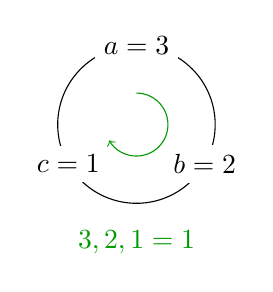
\begin{tikzpicture}
		\draw[black] (0, 0) circle (1);
		\node[rectangle, fill=white] at (90:1) {\(a = 3\)};
		\node[rectangle, fill=white] at (-30:1) {\(b = 2\)};
		\node[rectangle, fill=white] at (-150:1) {\(c = 1\)};
		\draw[->, green!60!black] (90:.4) arc (90:-150:.4);
		\node[green!60!black] at (0, -1.5) {\(\ind{3, 2, 1} = 1\)};
	\end{tikzpicture} \hspace{1cm}
	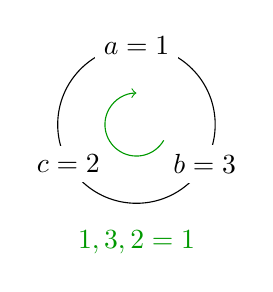
\begin{tikzpicture}
		\draw[black] (0, 0) circle (1);
		\node[rectangle, fill=white] at (90:1) {\(a = 1\)};
		\node[rectangle, fill=white] at (-30:1) {\(b = 3\)};
		\node[rectangle, fill=white] at (-150:1) {\(c = 2\)};
		\draw[->, green!60!black, rotate=-120] (90:.4) arc (90:-150:.4);
		\node[green!60!black] at (0, -1.5) {\(\ind{1, 3, 2} = 1\)};
	\end{tikzpicture} \hspace{1cm}
	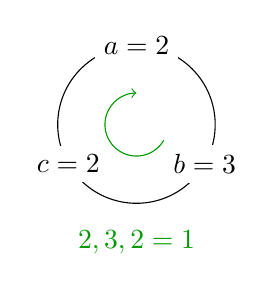
\begin{tikzpicture}
		\draw (0, 0) circle (1);
		\node[rectangle, fill=white] at (90:1) {\(a = 2\)};
		\node[rectangle, fill=white] at (-30:1) {\(b = 3\)};
		\node[rectangle, fill=white] at (-150:1) {\(c = 2\)};
		\draw[->, green!60!black, rotate=-120] (90:.4) arc (90:-150:.4);
		\node[green!60!black] at (0, -1.5) {\(\ind{2, 3, 2} = 1\)};
	\end{tikzpicture} \\
	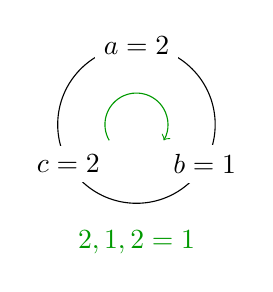
\begin{tikzpicture}
		\draw[black] (0, 0) circle (1);
		\node[rectangle, fill=white] at (90:1) {\(a = 2\)};
		\node[rectangle, fill=white] at (-30:1) {\(b = 1\)};
		\node[rectangle, fill=white] at (-150:1) {\(c = 2\)};
		\draw[->, green!60!black, rotate=120] (90:.4) arc (90:-150:.4);
		\node[green!60!black] at (0, -1.5) {\(\ind{2, 1, 2} = 1\)};
	\end{tikzpicture} \hspace{1cm}
	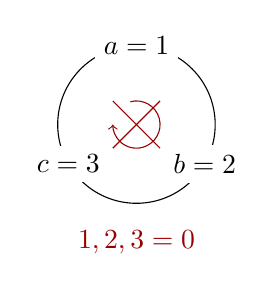
\begin{tikzpicture}
		\draw[black] (0, 0) circle (1);
		\node[rectangle, fill=white] at (90:1) {\(a = 1\)};
		\node[rectangle, fill=white] at (-30:1) {\(b = 2\)};
		\node[rectangle, fill=white] at (-150:1) {\(c = 3\)};
		\draw[->, red!60!black] (105:.3) arc (105:-180:.3);
		\draw[red!60!black] (.3,.3) -- (-.3,-.3);
		\draw[red!60!black] (.3,-.3) -- (-.3,.3);
		\node[red!60!black] at (0, -1.5) {\(\ind{1, 2, 3} = 0\)};
	\end{tikzpicture} \hspace{1cm}
	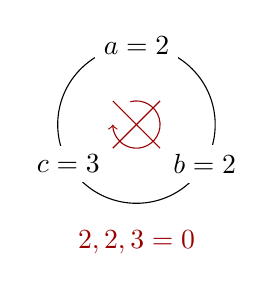
\begin{tikzpicture}
		\draw[black] (0, 0) circle (1);
		\node[rectangle, fill=white] at (90:1) {\(a = 2\)};
		\node[rectangle, fill=white] at (-30:1) {\(b = 2\)};
		\node[rectangle, fill=white] at (-150:1) {\(c = 3\)};
		\draw[->, red!60!black] (105:.3) arc (105:-180:.3);
		\draw[red!60!black] (.3,.3) -- (-.3,-.3);
		\draw[red!60!black] (.3,-.3) -- (-.3,.3);
		\node[red!60!black] at (0, -1.5) {\(\ind{2, 2, 3} = 0\)};
	\end{tikzpicture}
	\caption{Examples of the indicator function \(\ind{a, b, c}\) for an unsigned alphabet.}
	\label{fig:indicator}
\end{figure}

In signed alphabets, \(\ind{a, b, c}\) indicates whether \(a, b, c\) is cyclically decreasing, where the earlier of two equal positive entries is considered smaller than the later one, and the earlier of two equal negative entries is considered larger than the later one.

\section{Fillings} \label{sec:fillings}

\subsection{Non-augmented Fillings} \label{subsec:non-augmented-fillings}

The \vocab{(non-augmented) skyline diagram} of a composition
\(\alpha = \composition{\alpha_1, \ldots, \alpha_n}\)
is the set
\begin{equation*}
	\dg(\alpha) = \left\{ (i, r) \suchthat i \in \interval{n} \text{ and } r \in \interval{\alpha_i} \right\},
\end{equation*}
where the first coordinate indexes the columns and the second coordinate indexes the rows.
In \cref{subsec:augmented-fillings}, we will define the \vocab{augmented skyline diagram} of a composition, hence the optional term \emph{non-augmented} is used when the distinction is necessary.
The elements of \(\dg(\alpha)\) are called \vocab{boxes}.
We draw the box \((i, r)\) as a square in column \(i\) and row \(r\).
\Cref{fig:skyline} provides an example of a skyline diagram.

\begin{figure}[htbp]
	\centering
	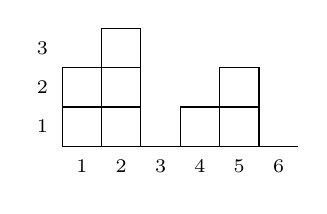
\begin{tikzpicture}[x=.5cm, y=.5cm]
		\foreach \height [count = \column] in {2, 3, 0, 1, 2, 0}{
				\foreach \row in {0,...,\height}{
						\ifnum \row = 0
							\path (\column, \row) rectangle (\column + 1, \row + 1);
							\draw (\column, \row+1) -- (\column + 1, \row + 1);
						\else
							\draw[black] (\column, \row) rectangle (\column + 1, \row + 1);
						\fi
					}
				\node at (\column + .5, .5) {\(\scriptstyle \column\)};
			}
		\foreach \row in {1, 2, 3}{
				\node at (.5, \row + .5) {\(\scriptstyle \row\)};
			}
	\end{tikzpicture}
	\caption{
		The skyline diagram 
		of the composition \(\alpha = \composition{2, 3, 0, 1, 2, 0}\).
	}
	\label{fig:skyline}
\end{figure}

A box \(u = (i_u, r_u)\) \vocab{attacks} \(v = (i_v, r_v)\) in \(\dg(\alpha)\) if
\(r_u = r_v\) and \(i_u < i_v\), that is, \(u\) and \(v\) are in the same row and \(u\) is to the left of \(v\); or
\(r_v = r_u - 1\) and \(i_v < i_u\), that is, \(u\) is in the row directly above \(v\) and \(u\) is to the right of \(v\).
\Cref{fig:attacking} illustrates the two configurations in which a box \(u\) attacks a box \(v\).
Let \(\Attack_{\dg(\alpha)}(u) \subset \dg(\alpha)\) be the set of boxes attacked by \(u\).
When there is no ambiguity, we may simply write \(\Attack(u)\).

\begin{figure}[htbp]
	\begin{equation*}
		\vcenter{\hbox{
				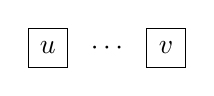
\begin{tikzpicture}[x=.5cm, y=.5cm]
					\draw[black] (0, 0) rectangle (1, 1);
					\node at (.5, .5) {\(u\)};
					\node at (2, .5) {\(\cdots\)};
					\draw[black] (3, 0) rectangle (4, 1);
					\node at (3.5, .5) {\(v\)};
				\end{tikzpicture}}}
		\qquad \text{or} \qquad
		\vcenter{\hbox{
				\begin{tikzpicture}[x=.5cm, y=.5cm]
					\draw[black, shift={(0,-.5)}] (0, 0) rectangle (1, 1);
					\node at (.5, .5-.5) {\(v\)};
					\node at (2, .5) {\(\cdots\)};
					\draw[black, shift={(0,.5)}] (3, 0) rectangle (4, 1);
					\node at (3.5, .5+.5) {\(u\)};
				\end{tikzpicture}}}.
	\end{equation*}
	\caption{Configurations in which a box \(u\) attacks a box \(v\): either in the same row (left), or in consecutive rows (right). }
	\label{fig:attacking}
\end{figure}

Let \(u = (i, r) \in \dg(\alpha)\).
The \vocab{leg set} of \(u\) is the set \(\Leg_{\dg(\alpha)}(u) \subset \dg(\alpha)\) of boxes above \(u\) in the same column, that is, \(\Leg_{\dg(\alpha)}(u) = \left\{ (i, r') \in \dg(\alpha) \suchthat r' > r \right\}\).
The \vocab{leg statistic} of \(u\) is defined as \(\leg_{\dg(\alpha)}(u) = \left|\Leg_{\dg(\alpha)}(u)\right| = \alpha_i - r\).
The \vocab{arm set} of \(u\) is the set \(\Arm_{\dg(\alpha)}(u) \subset \dg(\alpha)\) of boxes \(v\) attacked by \(u\) such that \(\leg_{\dg(\alpha)}(v) \leq \leg_{\dg(\alpha)}(u)\), that is,
\begin{equation*}
	\Arm_{\dg(\alpha)}(u) = \left\{ v \in \Attack_{\dg(\alpha)}(u) \suchthat \leg_{\dg(\alpha)}(v) \leq \leg_{\dg(\alpha)}(u) \right\}.
\end{equation*}
The \vocab{arm statistic} of \(u\) is defined as \(\arm_{\dg(\alpha)}(u) = \left|\Arm_{\dg(\alpha)}(u)\right|\).
When there is no ambiguity, we may simply write \(\Leg(u)\), \(\leg(u)\), \(\Arm(u)\), and \(\arm(u)\).
The box \vocab{south} of \(u = (i, r)\) is the box \(\south{u} = (i, r-1)\), that is, the box directly below \(u\).
If \(r > 1\), then \(\south{u} \in \dg(\alpha)\); while if \(r = 1\), then \(\south{u}\) is still defined (in row \(0\)),
but it is not in \(\dg(\alpha)\).
See \cref{fig:leg-arm} for an example of the leg set, arm set, and south of a box.

\begin{figure}[htbp]
    \centering
	\begin{tikzpicture}[x=.5cm, y=.5cm]
		\def\shape{4, 3, 3, 5, 5, 1, 4, 4, 4, 5, 3, 2, 4}
			\xdef\reading{0}
			\foreach \height [count = \column] in \shape{
				\foreach \row in {1,...,\height}{
						\pgfmathparse{int(\reading + 1)}
						\xdef\reading{\pgfmathresult}
						\coordinate (B\reading) at (\column, \row);
					}
			}
			\def\filling{
				{ },{y},{ },{ },
				{ },{z},{ },
				{ },{z},{ },
				{ },{y},{ },{ },{ },
				{ },{y},{ },{ },{ },
				{ },
				{ },{y},{ },{ },
				{ },{d},{u},{x},
				{ },{ },{z},{ },
				{ },{ },{y},{ },{ },
				{ },{ },{z},
				{ },{ },
				{ },{ },{z},{ }}

			\foreach \i [count = \j] in \filling {
				\if\i u
					\draw[fill=black] (B\j) rectangle ++(1, 1);
				\else\if\i z
						\draw[pattern color=cyan, pattern=horizontal lines] (B\j) rectangle ++(1, 1);
						\draw[pattern color=magenta, pattern=north east lines] (B\j) rectangle ++(1, 1);
					\else\if\i x
							\draw[pattern color=green!70!black, pattern=vertical lines] (B\j) rectangle ++(1, 1);
						\else\if\i d
								\draw[pattern color=yellow!50!black, pattern=dots] (B\j) rectangle ++(1, 1);
							\else\if\i y
									\draw[pattern color=cyan, pattern=horizontal lines] (B\j) rectangle ++(1, 1);
								\else
									\draw[fill=white] (B\j) rectangle ++(1, 1);
								\fi\fi\fi\fi\fi
			}

	\end{tikzpicture}
	\caption{
		The leg set (\,\raisebox{-.7ex}{\begin{tikzpicture}[x=.45cm, y=.45cm] \protect\draw[pattern color=green!70!black, pattern=vertical lines] (0, 0) rectangle ++(1, 1); \end{tikzpicture}}\,),
		the arm set (\,\raisebox{-.7ex}{\begin{tikzpicture}[x=.45cm, y=.45cm] \protect\draw[pattern color=magenta, pattern=north east lines] (0, 1) rectangle ++(1, 1); \end{tikzpicture}}\,),
		the attacked set (\,\raisebox{-.7ex}{\begin{tikzpicture}[x=.45cm, y=.45cm] \protect\draw[pattern color=cyan, pattern=horizontal lines] (0, 1) rectangle ++(1, 1); \end{tikzpicture}}\,),
		and the south (\,\raisebox{-.7ex}{\begin{tikzpicture}[x=.45cm, y=.45cm] \protect\draw[pattern color=yellow!50!black, pattern=dots] (1, 4) rectangle ++(1, 1); \end{tikzpicture}}\,)
		of the box \(u = (8, 3)\) (\,\raisebox{-.7ex}{
\begin{tikzpicture}[x=.45cm, y=.45cm] \protect\draw[fill=black] (5, 2) rectangle ++(1, 1); \end{tikzpicture}}\,)
		in the skyline diagram of \(\alpha = \composition{4, 3, 3, 5, 5, 1, 4, 4, 4, 5, 3, 2, 4}\) with \(\leg(u)=1\) and \(\arm(u)=5\).
	}
	\label{fig:leg-arm}
\end{figure}

A \vocab{filling} of shape \(\alpha = \composition{\alpha_1, \ldots, \alpha_n}\) with labels in an alphabet \(\mathcal{A}\) is a function \(T \colon \dg(\alpha) \to \mathcal{A}\).
Let \(\Fill[\mathcal{A}](\alpha)\) denote the set of fillings of shape \(\alpha\) with labels in \(\mathcal{A}\).
A filling \(T\in \Fill[\mathcal{A}](\alpha)\)
is \vocab{non-attacking} if \(T(u) \neq T(v)\) whenever \(u\) attacks \(v\) in \(\dg(\alpha)\).
Let \(\NAF[\mathcal{A}](\alpha) \subseteq \Fill[\mathcal{A}](\alpha)\) denote the set of non-attacking fillings of shape \(\alpha\) with labels in \(\mathcal{A}\).

The \vocab{content} of a filling \(T\) with labels in the unsigned alphabet \(\mathcal{A} = \interval{n}\) or \(\mathcal{A} = \positives\) is the composition \(\beta = \content(T)\) where \(\beta_i\) is the number of occurrences of the label \(i\) in \(T\).
The \vocab{content} of a filling \(T\) with labels in the signed alphabet \(\mathcal{A}_\pm = [n]_\pm\) or \(\mathcal{A}_\pm = \integers_\pm\) is the composition \(\beta = \content(T)\) where \(\beta_i\) is the number of occurrences of the label \(i\) or \(\bar{i}\) in \(T\), i.e., the number of entries of \(T\) whose absolute value is \(i\).
In both contexts, we let
\[
	\mathbf{x}^T = \mathbf{x}^{\content(T)} = \prod_{i} x_i^{\beta_i}.
\]

See \Cref{fig:non-attacking-filling} for an example of a non-attacking filling.

\begin{figure}[htbp]
    \centering
	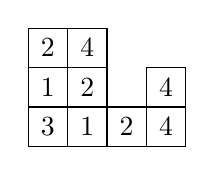
\begin{tikzpicture}[x=.5cm, y=.5cm]
		\def\shape{2, 2, 0, 1}
		\def\filling{
			3, 1, 2,
			1, 2, 4,
			2,
			4, 4}
		\edef\reading{0}
		\foreach \height [count = \column] in \shape{
			\foreach \row in {0,...,\height}{
					\pgfmathparse{int(\reading + 1)}
					\xdef\reading{\pgfmathresult}
					\draw[black] (\column, \row) rectangle (\column + 1, \row + 1);
					\coordinate (B\reading) at (\column + .5, \row + .5);
				}
		}
		\foreach \i [count = \j] in \filling{ \node at (B\j) {\i}; }
	\end{tikzpicture}
	\caption{
		A non-attacking filling of
		shape \(\alpha = \composition{3, 3, 1, 2}\)
		with \(\content(T) = \composition{2, 3, 1, 3}\).
	}
	\label{fig:non-attacking-filling}
\end{figure}

Recall that boxes in row \(0\), which are not in \(\dg(\alpha)\),
can be obtained as the south of boxes in row \(1\).
By convention, if \(w\) is a box in row \(0\),
then we define \(T(w) = \infty\).

Given a filling \(T \in \Fill(\alpha)\),
we say that a box \(u \in \dg(\alpha)\)
is a \vocab{descent} in \(T\) if \(\ind{T(u), T(\south{u})} = 1\).
Note that boxes in row \(1\) are never descents,
since the label of the south of a box in row \(1\) is always \(\infty\), by convention.
Let \(\Des(T) \subseteq \dg(\alpha)\) denote the set of descents in \(T\).
The \vocab{major index} of \(T\) is
\begin{equation*}
	\maj(T)
	= \sum_{u \in \Des(T)} \left( \leg(u) + 1 \right)
	= \sum_{u \in \dg(\alpha)} \ind{T(u), T(\south{u})} \left( \leg(u) + 1 \right).
\end{equation*}
See \cref{fig:major-index} for an example.
\begin{figure}[htbp]
    \centering
	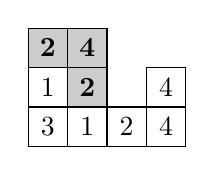
\begin{tikzpicture}[x=.5cm, y=.5cm]
		\def\shape{2, 2, 0, 1}
		\def\filling{
			3, 1, \textbf2,
			1, \textbf2, \textbf4,
			2,
			4, 4}
		\xdef\reading{0}
		\fill[black!20] (1,2) rectangle ++(1,1);
		\fill[black!20] (2,1) rectangle ++(1,1);
		\fill[black!20] (2,2) rectangle ++(1,1);
		\foreach \height [count = \column] in \shape{
			\foreach \row in {0,...,\height}{
					\pgfmathparse{int(\reading + 1)}
					\xdef\reading{\pgfmathresult}
					\draw[black] (\column, \row) rectangle (\column + 1, \row + 1);
					\coordinate (B\reading) at (\column + .5, \row + .5);
				}
		}
		\foreach \i [count = \j] in \filling{
			\node at (B\j) {\i};
		}
	\end{tikzpicture}
	\caption{
		The filling \(T\) above has three descents (shaded boxes).
		The leg statistics of the descents are: \(\leg(1,2)=\leg(2,2)=0\) and \(\leg(2,1)=1\).
		Thus, the major index of \(T\) is \(\maj(T) = 1 + 1 + 2 = 4\).
	}
	\label{fig:major-index}
\end{figure}

A \vocab{triple} is an ordered tuple \((u, v, w)\) of boxes
such that \(u \in \dg(\alpha)\), \(v \in \Arm(u)\), and \(w = \south{u}\).
The total number of triples in \(\dg(\alpha)\) is
\begin{equation*}
	\sum_{u \in \dg(\alpha)} \arm(u).
\end{equation*}
If \(v\) is to the right of \(u\) in the same row as \(u\),
then the triple is of \vocab{type A},
and if \(v\) is to the left of \(u\) in the row directly below \(u\),
then the triple is of \vocab{type B}.%
\footnote{This is not related to Cartan types \(A_n\) and \(B_n\).
In \cite{HHL08} and \cite{Fer11},
they are called \vocab{type II} and \vocab{type I}, respectively.}
The configurations of the boxes \(u\), \(v\), and \(w\)
when the tuple \((u, v, w)\) is of type A or type B are shown in \cref{fig:triples}.
Note that if \(\alpha\) is a partition, there are no triples of type B.
\begin{figure}[ht]
	\centering
	\begin{subfigure}[t]{0.45\textwidth}
		\centering
		\begin{ytableau}
			u & \none[\cdots] & v \\
			w
		\end{ytableau}
		\caption*{(\textsc{Type A})
		The column containing \(u\) and \(w\) is at least as high as the column containing \(v\).}
	\end{subfigure}\hspace{0.05\textwidth}
	\begin{subfigure}[t]{0.45\textwidth}
		\centering
		\begin{ytableau}
			\none & \none & u \\
			v & \none[\cdots] & w
		\end{ytableau}
		\caption*{(\textsc{Type B})
		The column containing \(u\) and \(w\) is strictly higher than the column containing \(v\).}
	\end{subfigure}
	\caption{Configurations for triples of type A (left) and type B (right).}
	\label{fig:triples}
\end{figure}

Note that the definition of a triple \((u, v, w)\) allows for \(u\) to be in row \(1\), and consequently for \(w\) to be in row \(0\).
A triple that has \(u\) in row \(1\) is called a \vocab{degenerate triple}.
A degenerate triple is always of type A, since \(v \in \Arm(u) \subset \dg(\alpha)\), and therefore cannot be in row \(0\).

% We define the \vocab{inversion} and \vocab{coinversion} statistics,
% following \cite[Section~3]{HHL08}.

Given a filling \(T \in \Fill(\alpha)\),
a triple \((u, v, w)\) in \(\dg(\alpha)\) is
an \vocab{inversion triple} if \(\ind{T(u), T(v), T(w)} = 1\),
and is a \vocab{coinversion triple} otherwise.
Let \(\inv(T)\) and \(\coinv(T)\) denote
the number of inversion triples and coinversion triples in \(T\),
respectively.
% We denote by \(\InversionTriples(T)\) and \(\CoinversionTriples(T)\) the sets of inversion triples and coinversion triples in \(T\), respectively, so that \(\inv(T) = |\InversionTriples(T)|\) and \(\coinv(T) = |\CoinversionTriples(T)|\).
% It is straightforward to check that these definitions of inversion triples
% are equivalent to those in \cite{Ale19} and \cite{CMW22}.
We have
\begin{equation} \label{eq:inv-plus-coinv}
	\inv(T) + \coinv(T) = \sum_{u \in \dg(\alpha)} \arm(u),
\end{equation}
the total number of triples in \(\dg(\alpha)\).
See \cref{fig:inversion-coinversion} for an example.

\begin{figure}[htbp]
    \centering
	\ytableausetup{boxsize=0.5cm}
	\colorlet{inversion}{orange!70!white}
	\colorlet{coinversion}{purple!50!white}
	\renewcommand{\arraystretch}{1.5}
	\begin{tabular}{ccccc}
		\begin{ytableau}
			*(coinversion) \textbf2 & *(coinversion) \textbf4 \\
			*(coinversion) \textbf1 & 2 & \none & 4 \\
			3 & 1 & 2 & 4
		\end{ytableau}
		&
		\begin{ytableau}
			2 & 4 \\
			*(coinversion) \textbf1 & *(coinversion) \textbf2 & \none & 4 \\
			*(coinversion) \textbf3 & 1 & 2 & 4
		\end{ytableau}
		&
		\begin{ytableau}
			2 & 4 \\
			*(inversion) \textbf1 & 2 & \none & *(inversion) \textbf4 \\
			*(inversion) \textbf3 & 1 & 2 & 4
		\end{ytableau}
		&
		\begin{ytableau}
			2 & 4 \\
			1 & *(coinversion) \textbf2 & \none & *(coinversion) \textbf4 \\
			3 & *(coinversion) \textbf1 & 2 & 4
		\end{ytableau}
		&
		\begin{ytableau}
			2 & 4 \\
			1 & 2 & \none & *(inversion) \textbf4 \\
			3 & 1 & *(inversion) \textbf2 & *(inversion) \textbf4
		\end{ytableau}
		\\
		\(\ind{2, 4, 1} = 0\)
		&
		\(\ind{1, 2, 3} = 0\)
		&
		\(\ind{1, 4, 3} = 1\)
		&
		\(\ind{2, 4, 1} = 0\)
		&
		\(\ind{4, 2, 1} = 1\)
	\end{tabular}
	\caption{
		We show all five triples of
		the filling \(T\) in \cref{fig:non-attacking-filling};
		the first four are of type A, and the last one is of type B.
		There are two inversion triples (orange)
		and three coinversion triples (purple),
		which gives \(\inv(T) = 2\) and \(\coinv(T) = 3\).
	}
	\label{fig:inversion-coinversion}
\end{figure}

There is another interpretation of \(\inv(T)\) and \(\coinv(T)\), in terms of inversion pairs.
An \vocab{inversion pair} in a filling \(T\) is a pair \(\{u, v\}\) of boxes in \(\dg(\alpha)\) such that \(u\) attacks \(v\) and \(\ind{T(u), T(v)} = 1\).
Let \(\InversionPairs(T)\) denote the set of inversion pairs in \(T\).

\begin{proposition}[{\cite[739]{HHL05}}] \label{prop:inv-via-inversion-pairs}
	Let \(T \in \Fill(\alpha)\).
	Then
	\begin{equation*}
		\inv(T) = \left|\InversionPairs(T)\right| - \sum_{u \in \Des(T)} \arm(u).
	\end{equation*}
\end{proposition}

\todo{Write short proof of alternate description of \(\inv(T)\).}

\Cref{prop:inv-via-inversion-pairs} gives an alternative description of \(\inv(T)\).
Together with \Cref{eq:inv-plus-coinv}, we also obtain an alternative description of \(\coinv(T)\) by
\begin{equation*}
	\coinv(T) = \sum_{u \in \dg(\alpha)} \arm(u) - \inv(T)
	= \sum_{u \in \dg(\alpha) \setminus \Des(T)} \arm(u) - \left|\InversionPairs(T)\right|.
\end{equation*}

\subsection{Augmented Fillings} \label{subsec:augmented-fillings}

In the context of augmented fillings,
we either take the unsigned alphabet \(\mathcal{A} = \interval{n}\),
or the signed alphabet \(\mathcal{A}_\pm = [n]_\pm\).

The \vocab{augmented skyline diagram} of a composition
\(\alpha = \composition{\alpha_1, \ldots, \alpha_n}\)
is the set
\begin{equation*}
	\adg(\alpha) = \dg(\alpha) \cup \{(i, 0) \suchthat i \in \interval{n}\},
\end{equation*}
where the first coordinate indexes the columns and the second coordinate indexes the rows.
The boxes in row \(0\) are collectively called the \vocab{basement}.

The attacking relation, leg set, arm set, leg statistic, arm statistic in \(\adg(\alpha)\) are defined as in \cref{subsec:non-augmented-fillings}.
For these definitions, the boxes in row \(0\) of \(\adg(\alpha)\) behave just like the other boxes in \(\adg(\alpha)\).

Since boxes in row \(0\) are now part of the diagram, subtle differences arise.
For example, for \(u = (i, r) \in \adg(\alpha)\),
we have \(\Attack_{\adg(\alpha)}(u) = \Attack_{\dg(\alpha)}(u)\) if \(r \geq 2\).
However, if \(r = 1\), then \(\Attack_{\adg(\alpha)}(u)\) may contain boxes in row \(0\) that are not in \(\Attack_{\dg(\alpha)}(u)\).
A similar comment applies to \(\Arm_{\adg(\alpha)}(u)\) and \(\Arm_{\dg(\alpha)}(u)\), and consequently to \(\arm_{\adg(\alpha)}(u)\) and \(\arm_{\dg(\alpha)}(u)\).
Therefore, one must pay attention to which diagram is being used when computing these sets and statistics for a box in row \(1\).

The definition of the south of a box is slightly different in the augmented setting.
Given a box \(u = (i, r)\), if \(r \geq 1\), the \vocab{south} of \(u\) is the box \(\south{u} = (i, r-1)\), while if \(r = 0\), then \(\south{u}\) is not defined.
Note that the south of a box in row \(1\) of \(\adg(\alpha)\) is also a box in \(\adg(\alpha)\), unlike in \Cref{subsec:non-augmented-fillings} where the south of a box in row \(1\) is not in \(\dg(\alpha)\).
We also remark that the south of a box in row \(0\) is not a box in row \(-1\) outside \(\adg(\alpha)\), but rather is simply undefined.

An \vocab{augmented filling} of shape \(\alpha = \composition{\alpha_1, \ldots, \alpha_n}\), basement \(\sigma = \composition{\sigma_1, \ldots, \sigma_n}\), and labels in an alphabet \(\mathcal{A}\) is a function \(T \colon \adg(\alpha) \to \mathcal{A}\) such that \(T(i, 0) = \sigma_i\) for all \(i \in \interval{n}\).

Let \(\Fill[\mathcal{A}](\alpha, \sigma)\) denote the set of augmented fillings of shape \(\alpha\), basement \(\sigma\), and labels in \(\mathcal{A}\).
The non-attacking condition for augmented fillings is defined as in \cref{subsec:non-augmented-fillings}.
Let \(\NAF[\mathcal{A}](\alpha, \sigma) \subseteq \Fill[\mathcal{A}](\alpha, \sigma)\) denote the set of non-attacking augmented fillings of shape \(\alpha\), basement \(\sigma\), and labels in \(\mathcal{A}\).

Note that the non-attacking condition implies that the basement \(\sigma\) of a non-attacking augmented filling with labels in \(\interval{n}\) is a permutation of \(\interval{n}\).
For (possibly attacking) augmented fillings with labels in \(\interval{n}\) or \(\interval{n}_\pm\), the definition allows for repeated or negative entries in the basement.
However, the applications in this work only require the case of a permutation basement, that is, positive and distinct entries in the basement.

The definitions of content, descents, and major index for augmented fillings are as in \cref{subsec:non-augmented-fillings}.
Note that boxes in row \(1\) can be descents, since the label of the south of a box in row \(1\) is now given by the basement, rather than being \(\infty\) by convention.
However, boxes in row \(0\) are never descents, since they do not have a south.

A triple \((u, v, w)\) is defined as in \cref{subsec:non-augmented-fillings}.
Since boxes in row \(0\) do not have a south, \(u\) cannot be in row \(0\).
There is no concept of a degenerate triple in augmented fillings.
The definitions of inversion triples, coinversion triples, and the statistics \(\inv(T)\) and \(\coinv(T)\) for augmented fillings are as in \cref{subsec:non-augmented-fillings}.
In the augmented setting, the total number of triples in \(\adg(\alpha)\) is
\begin{equation} \label{eq:total-triples-augmented}
	\sum_{u \in \dg(\alpha)} \arm_{\adg(\alpha)}(u)
\end{equation}
Note that this sum does not include boxes \(u\) in row \(0\).
We remark that this sum may be different from \(\sum_{u \in \dg(\alpha)} \arm_{\dg(\alpha)}(u)\) from \cref{subsec:non-augmented-fillings}, since the arm statistic for boxes in row \(1\) may be different in the two settings.

Similarly to \cref{subsec:non-augmented-fillings},
there is another interpretation of \(\inv(T)\) and \(\coinv(T)\), in terms of inversion pairs.
An \vocab{inversion pair} in an augmented filling \(T\) is a pair \(\{u, v\}\) of boxes with \(u \in \dg(\alpha)\) and \(v \in \adg(\alpha)\) such that \(u\) attacks \(v\) and \(\ind{T(u), T(v)} = 1\).
Let \(\InversionPairs(T)\) denote the set of inversion pairs in \(T\).

\begin{proposition}[{\cite[739]{HHL05}}] \label{prop:inv-via-inversion-pairs-augmented}
	Let \(T \in \Fill(\alpha)\).
	Then
	\begin{equation*}
		\inv(T) = \left|\InversionPairs(T)\right| - \sum_{u \in \Des(T)} \arm(u).
	\end{equation*}
\end{proposition}

\todo{Write short proof of alternate description of \(\inv(T)\).}

\Cref{prop:inv-via-inversion-pairs-augmented} gives an alternative description of \(\inv(T)\).
Together with \Cref{eq:total-triples-augmented}, we also obtain an alternative description of \(\coinv(T)\) by
\begin{equation*}
	\coinv(T) = \sum_{u \in \dg(\alpha)} \arm(u) - \inv(T)
	= \sum_{u \in \dg(\alpha) \setminus \Des(T)} \arm(u) - \left|\InversionPairs(T)\right|.
\end{equation*}


\section{Combinatorial models for Macdonald polynomials}

\subsection{Modified Macdonald polynomials \texorpdfstring{\(\tilde{H}_\mu\)}{H̃μ} as tableaux generating functions}

Recall that the Modified Macdonald polynomials \(\tilde{H}_\mu\) are a family of polynomials indexed by partitions \(\mu\).

In \cite{HHL05}, \citeauthor{HHL05} give a combinatorial formula for \(\tilde{H}_\mu\) as 
\begin{equation}
	\tilde{H}_\mu(\mathbf{x}; q, t) =
	\sum_{T \in \Fill[\positives](\mu)} q^{\inv(T)} t^{\maj(T)} \mathbf{x}^T,
\end{equation}
where \(\Fill[\positives](\mu)\) is the set of fillings of shape \(\mu\) with labels in the positive integers \(\positives\).

In \cite{HHL08}, \citeauthor{HHL08} show that the set may be changed to \(\Fill[\positives](\alpha)\) for any rearrangement \(\alpha\) of \(\mu\), and the formula still holds.
\todo{Add sentence on that this will be showed again in \Cref{chap:bijective}.}

\subsection{Integral form symmetric Macdonald polynomials \texorpdfstring{\(J_\mu\)}{Jμ} as tableaux generating functions}

Recall that the integral form Macdonald polynomials \(J_\mu\) are a family of polynomials indexed by partitions \(\mu\).

There are three closely related tableaux formulas for \(J_\mu\):
one over all fillings using the signed alphabet \(\interval{n}_\pm\),
\begin{equation} \label{eq:J-Fill-signed}
	J_\mu(\mathbf{x}; q, t)
	= \sum_{T \in \Fill[\interval{n}_\pm](\mu)} \mathbf{x}^T
	q^{\maj(T)}
	t^{\coinv(T)}
	(-t)^{\operatorname{neg}(T)},
\end{equation}
where \(\operatorname{neg}(T)\) denotes the number of negative entries in \(T\);
one over all non-attacking fillings using the signed alphabet \(\interval{n}_\pm\),
\begin{equation} \label{eq:J-NAF-signed}
	J_\mu(\mathbf{x}; q, t)
	= \sum_{T \in \NAF[\interval{n}_\pm](\mu)} \mathbf{x}^T
	q^{\maj(T)}
	t^{\coinv(T)}
	(-t)^{\operatorname{neg}(T)};
\end{equation}
and another one over all non-attacking fillings using the unsigned alphabet \(\interval{n}\),
\begin{equation} \label{eq:J-NAF-unsigned}
	J_\mu(\mathbf{x}; q, t)
	= \sum_{T \in \NAF[\interval{n}](\mu)} \mathbf{x}^T
	q^{\maj(T)} t^{\coinv(T)}
	\prod_{\substack{u \in \dg(\mu) \\ T(u) = T(\south{u})}}
	(1 - q^{1 + \leg(u)} t^{1 + \arm(u)})
	\prod_{\substack{u \in \dg(\mu) \\ T(u) \neq T(\south{u})}}
	(1 - t)
\end{equation}

The equivalence between equations \Cref{eq:J-Fill-signed} and \Cref{eq:J-NAF-signed} is obtained via a sign-reversing involution on the set of attacking signed fillings.
The equivalence between equations \Cref{eq:J-NAF-signed} and \Cref{eq:J-NAF-unsigned} is obtained by grouping all signed fillings that differ only by signs.

\todo{Properly cite \cite{HHL05} with correct section/theorem/equation number.}

\subsection{Symmetric Macdonald polynomials \texorpdfstring{\(P_\mu\)}{Pμ} as tableaux generating functions}

Recall that the symmetric Macdonald polynomials \(P_\mu\) are a family of polynomials indexed by partitions \(\mu\).
The integral form Macdonald polynomials \(J_\mu\) is a scalar multiple of \(P_\mu\), with relationship given by
\begin{equation}
	J_\mu(\mathbf{x}; q, t)
	=
	\left(
		\prod_{u \in \dg(\mu)} (1 - q^{1 + \leg(u)} t^{\arm(u)})
	\right)
	P_\mu(\mathbf{x}; q, t)
	.
\end{equation}
Therefore, from \Cref{eq:J-NAF-unsigned}, we obtain a tableaux formula for \(P_\mu\) as
\begin{equation} \label{eq:P-NAF-unsigned}
	P_\mu(\mathbf{x}; q, t)
	= \sum_{T \in \NAF[\interval{n}](\mu)} \mathbf{x}^T
	q^{\maj(T)} t^{\coinv(T)}
	\prod_{\substack{u \in \dg(\mu) \\ T(u) \neq T(\south{u})}}
	\frac{1 - t}{1 - q^{1 + \leg(u)} t^{1 + \arm(u)}}.
\end{equation}

\todo{Add a reference for the scaling factor.}

\subsection{Permuted-basement nonsymmetric Macdonald polynomials \texorpdfstring{\(E_\alpha^\sigma\)}{Eασ} as tableaux generating functions}
\label{sec:tableau-formula}

Recall that the permuted-basement nonsymmetric Macdonald polynomials \(E_\alpha^\sigma\) are a family of polynomials indexed by a composition \(\alpha\) and a permutation \(\sigma\).

\cite[Definition~4.4.2]{Fer11} give a tableau formula for permuted-basement Macdonald polynomials \(E_\alpha^\sigma\) as
\begin{equation} \label{eq:E-NAF-unsigned}
	E^{\sigma}_{\alpha}(\mathbf{x}; q, t) =
	\sum_{T \in \NAF(\alpha, \sigma)}
	\mathbf{x}^{\content(T)}
	q^{\maj(T)} t^{\coinv(T)}
	\prod_{\substack{u \in \dg(\alpha) \\ T(u) \neq T(\south{u})}}
	\frac{1 - t}{1 - q^{1 + \leg(u)} t^{1 + \arm(u)}}.
\end{equation}

\subsection{Integral form permuted-basement nonsymmetric Macdonald polynomials \texorpdfstring{\(\mathcal{E}_\alpha^\sigma\)}{Eασ} as tableaux generating functions}

Recall that the integral form permuted-basement nonsymmetric Macdonald polynomials \(\mathcal{E}_\alpha^\sigma\) are a family of polynomials indexed by a composition \(\alpha\) and a permutation \(\sigma\).
The integral form permuted-basement nonsymmetric Macdonald polynomials \(\mathcal{E}_\alpha^\sigma\) is a scalar multiple of \(E_\alpha^\sigma\), with relationship given by
\begin{equation}
	\mathcal{E}_\alpha^\sigma(\mathbf{x}; q, t)
	=
	\left(
		\prod_{u \in \dg(\alpha)} (1 - q^{1 + \leg(u)} t^{\arm(u)})
	\right)
	E_\alpha^\sigma(\mathbf{x}; q, t).
\end{equation}
Therefore, from \Cref{eq:E-NAF-unsigned}, we obtain a tableaux formula for \(\mathcal{E}_\alpha^\sigma\) as
\begin{equation} \label{eq:calE-NAF-unsigned}
	\mathcal{E}^{\sigma}_{\alpha}(\mathbf{x}; q, t) =
	\sum_{T \in \NAF(\alpha, \sigma)}
	\mathbf{x}^{\content(T)}
	q^{\maj(T)} t^{\coinv(T)}
	\prod_{\substack{u \in \dg(\alpha) \\ T(u) \neq T(\south{u})}}
	(1 - q^{1 + \leg(u)} t^{1 + \arm(u)})
	\prod_{\substack{u \in \dg(\alpha) \\ T(u) \neq T(\south{u})}}
	(1 - t).
\end{equation}

Using similar methods as in \cite{HHL05} (in reverse order),
we can obtain two similar equations for \(\mathcal{E}_\alpha^\sigma\).
One over all non-attacking augmented fillings using the unsigned alphabet \(\interval{n}\),
\begin{equation} \label{eq:calE-NAF-signed}
	\mathcal{E}^{\sigma}_{\alpha}(\mathbf{x}; q, t) =
	\sum_{T \in \NAF[\interval{n}](\alpha, \sigma)}
	\mathbf{x}^{\content(T)}
	q^{\maj(T)} t^{\coinv(T)}
	(-t)^{\operatorname{neg}(T)};
\end{equation}
and one over all augmented fillings using the signed alphabet \(\interval{n}_\pm\),
\begin{equation} \label{eq:calE-Fill-signed}
	\mathcal{E}^{\sigma}_{\alpha}(\mathbf{x}; q, t) =
	\sum_{T \in \Fill[\interval{n}_\pm](\alpha, \sigma)}
	\mathbf{x}^{\content(T)}
	q^{\maj(T)} t^{\coinv(T)}
	(-t)^{\operatorname{neg}(T)}.
\end{equation}